\section{Evaluation der Implementation mit echten Logdateien}
In diesem Abschnitt präsentieren wir unsere Implementierung für die Analyse von \gls{ssh}-Logdateien der Hochschule. 

Die Extrahierung des Inhalts der Logdateien erfolgt im Promtail mit folgenden Konfigurationen:
\begin{table}[H]
    \setstretch{1}
    \begin{tabularx}{\textwidth}{|m{5.5cm}|X|}
    \hline
    \multicolumn{1}{|c|}{\textbf{Konfigurationsfeld}} & \multicolumn{1}{|c|}{\textbf{Beschreibung}} \\
    \hline
    \textbf{scrape\_configs} & Steht für die Funktionalität von Promtail, automatisch nach Logdateien zu suchen. \\
    \hline
    - job\_name: sshlogs & Definition des Names unseres \quotes{job} \\
    \hline
    \textbf{pipeline\_stages:} & Diese Konfigurationen führen Änderungen in jeder Logzeile durch, die zum Loki geschickt wird. \\

    \hphantom{te}- match: \newline
    \hphantom{tex}selector: '\{job=``sshlogs''\}' \newline
    \hphantom{tex} action: keep \newline & Nur Logzeilen mit diesem \quotes{label} werden modifiziert und dessen Inhalt wird beibehalten. Alternativ gibt es \quotes{drop}, um diesen Inhalt zu löschen. \\

    \hphantom{tex}\textbf{stages:}  \newline
    \hphantom{tex}- regex: \newline
    \hphantom{text}expression:  \verb|`^(?P<time>[A-Za-z]|
                 \verb|{3}\s{1,2}\d{1,2}\s|
                 \verb|\d{2}:\d{2}:\d{2})*'| \newline
    \hphantom{tex}- timestamp: \newline
    \hphantom{text}source: time \newline
    \hphantom{text}format: ``Jan \_2 15:04:05'' \newline
    \hphantom{text}location: \quotes{Europe/Berlin} & Promtail bietet verschiedene Typen von \quotes{stages}, um die Logzeile zu bearbeiten. Diese werden nacheinander verarbeitet. Wir benutzen die \quotes{stages} \gls{RegExp} und dann \quotes{timestamp}. Der erste liest den Zeitstempel aus der \gls{ssh}-Logdatei aus, damit der zweite ihn verarbeiten und zu der von uns ausgewählten Format umwandeln kann. Schließlich speichert Loki den Zeitstempel der Zeile de Logdatei und nicht denen von des Hochladen in Loki. \\
    \hline
    \textbf{decompression} \newline
    \hphantom{te}enabled: true \newline
    \hphantom{te}initial\_sleep: 10s \newline
    \hphantom{te}format: gz & Promtail kann verschiedene Komprimierungsformate verarbeiten, darunter auch .gz, welches wir in unserer Arbeit verwenden. Das Feld \textit{initial\_sleep} beschreibt das Intervall, bevor die Dekomprimierung beginnt. Dieses Feld kann nützlich sein, wenn komprimierte Dateien vorhanden sind, deren Komprimierungsvorgang jedoch noch nicht abgeschlossen ist. Das Feld \textit{format} gibt das Komprimierungsformat an \citep{Grafana_Promtail}. \\  \hline

    \end{tabularx}
\end{table}

\begin{table}[H]
  \setstretch{1}
  \begin{tabularx}{\textwidth}{|m{5.5cm}|X|}
  \hline
  \multicolumn{1}{|c|}{\textbf{Konfigurationsfeld}} & \multicolumn{1}{|c|}{\textbf{Beschreibung}} \\
  \hline
  \textbf{static\_configs:} \newline
  \hphantom{te}- targets: \newline
  \hphantom{te}- loki \newline
  \hphantom{te}labels: \newline
  \hphantom{te}job: sshlogs \newline
  \hphantom{te}instance: \gls{Endpoint}-Name \newline
  \hphantom{te}\_\_path\_\_: /var/log/**.gz & Das Feld \textit{targets} bezieht sich auf die Kommunikation mit der Loki-Instanz. Das Feld \textit{labels} zeigt an, unter welcher Bezeichnung der Inhalt dieser Datei in Loki aufgerufen werden kann. \textit{\_\_path\_\_} gibt den Pfad zur Datei im System an.\\
  \hline
  \end{tabularx}
  \caption[Konfigurationsausschnitt von Promtail]
  {Konfigurationsausschnitt von Promtail}
  \label{tab:KonfigPromtail}
\end{table}

Unsere gesamte Einstellung für Promtail befindet sich im Anhang \ref{appendix:AngepasstGrafana} auf der Seite \pageref{appendix:AngepasstGrafana}.


%%% bearbeiten 

Unsere Logdateien haben eine Größe von ungefähr vier Megabyte, was im Vergleich zu produktiven Umgebungen, in denen Logdateien den Terabyte-Bereich erreichen können, gering ist. 


Trotz dieser Größe war unsere Synchronisierung nicht immer so präzise wie erwartet. Einige Abfragen, die bei der Implementierung mit 40 KB Logdateien einwandfrei funktionierten, führten hier zu folgender Fehlermeldung:

{\setstretch{1.0}
\begin{Verbatim}[fontsize=\small, frame=single]
maximum of series (500) reached for a single query  
\end{Verbatim}
}

Die offizielle Dokumentation und die verschiedenen Foren konnten uns keine endgültige Lösung mit der neuesten Version von Loki (2.8.2) bieten. Die verschiedenen Kombinationen in der Konfigurationsdatei von Loki führten immer zum selben Ergebnis. Zum Zeitpunkt unserer Arbeit (19.5.2022) haben wir versucht, über das GitHub-Forum Kontakt mit dem Grafana Loki-Team aufzunehmen, um mögliche Lösungsansätze zu finden.

Mit der Verwendung der Version 2.4.1 konnten wir die oben genannte Situation teilweise lösen. Unsere Abfragen wurden erfolgreich gesendet und die Diagramme wurden generiert. Der folgende Ausschnitt der Loki-Konfiguration in Tabelle \ref{tab:KonfigLoki} half dabei, die Leistungsparameter der Anwendung zu definieren:

%für diesen testlauf diese konfig aus diesem und diesem grund

\begin{table}[H]
  \setstretch{1}
  \begin{tabularx}{\textwidth}{|p{7cm}|X|}
  \hline
  \multicolumn{1}{|c|}{\textbf{Konfigurationsfeld}} & \multicolumn{1}{|c|}{\textbf{Beschreibung}} \\ \hline
  \textbf{limits\_config:} & Festlegung der Aufnahmerate; \\
  \hphantom{10}reject\_old\_samples: true & Aufnahme von alten Proben;\\ 
  \hphantom{10}reject\_old\_samples\_max\_age: 168h & Aufnahme von alten Proben, wenn sie älter als dieser Wert sind;\\
  \hphantom{10}ingestion\_rate\_mb: 1024 & Aufnahmerate in Megabyte pro Sekunde;\\ 
  \hphantom{10}ingestion\_burst\_size\_mb: 1024 & Aufnahmerate bei einer einzigen Weiterleitung in Megabyte; \\ 
  \hphantom{10}ingestion\_rate\_strategy: local &  Aufnahmerate wird entweder \quotes{local} definiert oder auf \quotes{global} aufgeteilt;  \\ 
  \hphantom{10}per\_stream\_rate\_limit: 12MB & Aufnahmerate in Byte pro Sekunde und pro Stream; \\ 
  \hphantom{10}max\_query\_series: 100000 & Maximale Anzahl von einzelnen Serien pro Abfrage; \\ 
  \hphantom{10}max\_query\_parallelism: 32 & Maximale Anzahl von parallelen Abfragen; \\ 
  \hphantom{10}split\_queries\_by\_interval: 24h & Trennung von Abfragen nach einem definierten Intervall;;\\ 
  \hphantom{10}max\_query\_length: 0h & Grenze für die Ausführungszeit. Dadurch wird eine Überlastung der Rechenkapazität vermieden; \\ 
  \bottomrule
  \end{tabularx}
\end{table}

\begin{table}[H]
  \setstretch{1}
  \begin{tabularx}{\textwidth}{|b{7cm}|X|}
  \hline
  \multicolumn{1}{|c|}{\textbf{Konfigurationsfeld}} & \multicolumn{1}{|c|}{\textbf{Beschreibung}} \\ \hline
  \textbf{querier:} & Einstellung für die Abfrage; \\ 
  \hphantom{10}max\_concurrent: 2048 & Anzahl der gleichzeitigen Abfragen;\\ \hline
  \textbf{frontend:} & Einstellung für die Abfrage im \gls{frontend};\\
  \hphantom{10}compress\_responses: true &Komprimierung der \gls{http}-Antworten;\\
  \hphantom{10}scheduler\_worker\_concurrency: 20 &  Anzahl der gleichzeitigen Abfragen, die verarbeitet werden; \\  \hline
  \textbf{table\_manager:} & Verwaltung der Vorratsdatenspeicherung;\\ 
  \hphantom{10}retention\_deletes\_enabled: false & Löschen von Tabellen in der Datenbank;\\ 
  \hphantom{10}retention\_period 360s & Tabellen werden gelöscht, wenn sie älter als dieser Wert sind;\\ \hline
  \end{tabularx}
  \caption[Konfigurationsausschnitt für Loki]
  {Konfigurationsausschnitt für Loki}
  \label{tab:KonfigLoki}
\end{table}

Trotz dieser Situation waren wir in der Lage, eine allgemeine Warnmeldung für eine hohe Anzahl von fehlgeschlagenen Anmeldeversuchen zu implementieren. Diese Warnmeldung ermöglicht es uns, potenzielle Sicherheitsbedrohungen zu erkennen und angemessen darauf zu reagieren.



% \newpage
% \newgeometry{right=30mm, left=30mm} 
% \thispagestyle{lscape}
% \begin{landscape}
%    Nach manuellen Aktualiserung sah unsere Graphik so aus:
%     \begin{figure}[H]
%        % \centering
%         \centerline{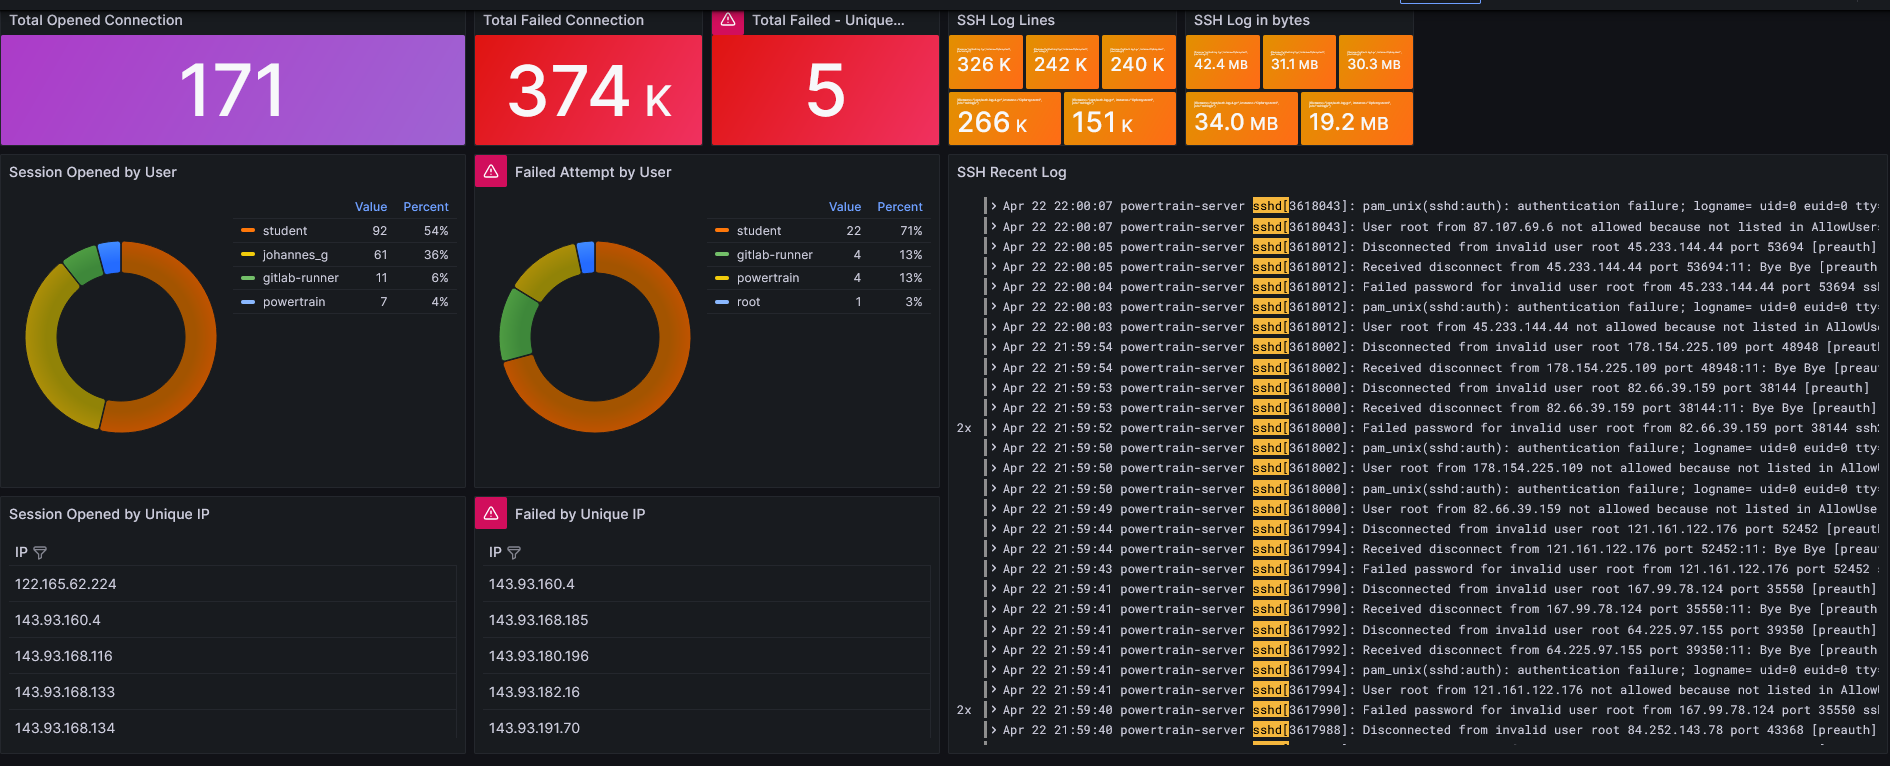
\includegraphics[width=1.8\textwidth]{assets/unserssh}}
%         %\includegraphics[width=1.2\textwidth]{assets/5.4.2_1_Abb.jpeg}
%         \caption[Ausgabe in Grafana von unseren \gls{ssh} Logdateien]
%         {Ausgabe in Grafana von unseren \gls{ssh} Logdateien}
%         \label{fig:Unserssh}
%         \centering
%     \end{figure} 
% \end{landscape}
% \restoregeometry


